\documentclass{article}
\usepackage[utf8]{inputenc}

\title{Decision Trees}
\author{Sylesh Suresh }
\date{July 2017}

\usepackage{graphicx}
\usepackage{minted}
\begin{document}

\maketitle

\section{Introduction}
Decision trees are powerful and interpretable classifiers that mirror human decisions unlike many other classifiers in supervised machine learning and are the building blocks of random forests. 
\section{Definition}
In essence, decision trees asks a series of true/false questions to narrow down what class a particular sample is. Here is an example of a decision tree one might use in real life to decide upon an activity on a given day:

\begin{figure}[h!]
\centering
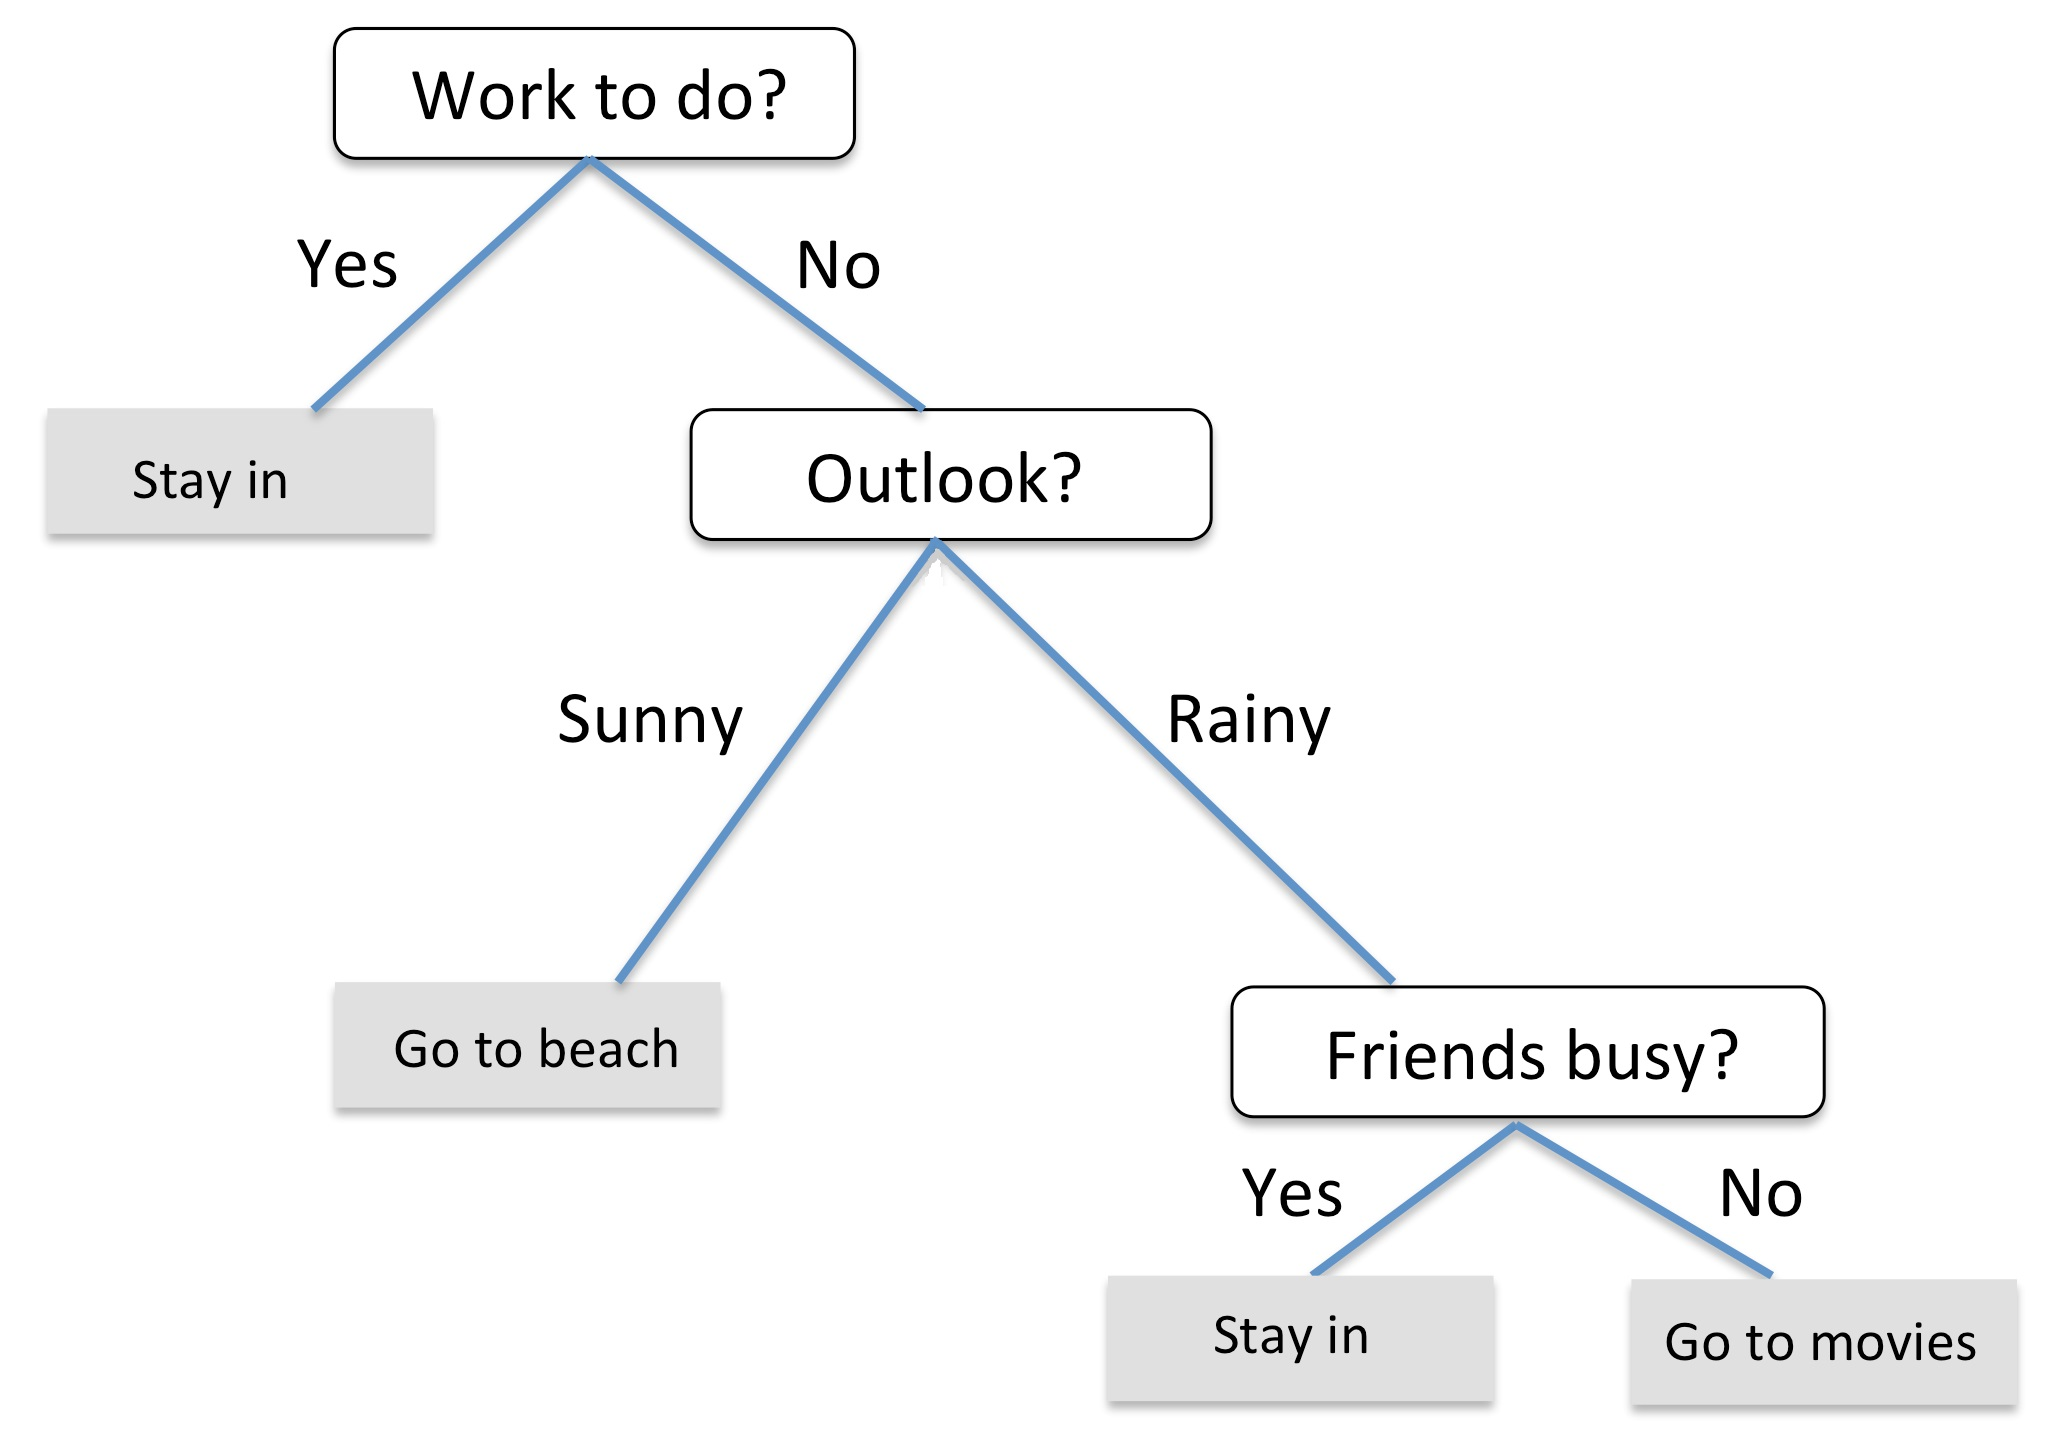
\includegraphics[scale=0.2]{dtree.jpg}
\caption{Real Life Decision Tree}
\label{fig:decisiontree}
\end{figure}

Although this figure asks categorical variable-based questions, we can ask numerical-based questions like \("x_1 < 5?"\) when the features are continuous. To build our tree, we start at the root node and ask a question that splits the data based on the feature such that the information gain is maximized. We continuously do this for each node until the decision tree can classify all the training data. Note that in practice this leads to overfitting, so the tree is usually pruned, i.e. a limit on the depth of the tree is set. 

\subsection{Information Gain}
We split each node on the feature that yields the most information gain. The formula for information gain in a binary decision tree is as follows:

\[IG(D_p, f) = I(D_p) - \frac{N_{left}}{N_p}I(D_{left}) - \frac{N_{right}}{N_p}I(D_{right}) \]

$D_p$ is the dataset of the parent node (the node which we are splitting), $f$ is the feature of the dataset which we are splitting on, $N_p$ is the total number of samples in the parent node, $N_{left}$ and $N_{right}$ are the number of samples in the datasets of the left child node and right child node respectively, and $I$ is the impurity measure. A node is pure if all samples in its dataset belong to the same class and is most impure when an equal number of samples belong to each class. Essentially, information gain calculates the difference between the impurity of the parent node and the impurity of the child nodes.

One commonly used measure of impurity is Gini impurity:

\[I_G(i) = 1 - \sum_{k=1}^{c} p(k|i)^2 \]

$p(k|i)$ is the proportion of samples of class \(k\) to the total number of samples in the dataset of the $i^{th}$ node.
The impurity is maximized when the classes of the node are perfectly mixed (for this example, consider a situation in which there are 2 classes, meaning c = 2):
\[1 - \sum_{k=1}^{c} 0.5^2 = 0.5\]

An alternative impurity measure is entropy, which is defined as:

\[-\sum_{k=1}^{c} p(k|i)log_2{p(k|i)} \]

Note that this function has a maximum of 1.0, not 0.5. In practice, Gini impurity and entropy yield similar results, so it is more useful to test different pruning cut-offs rather than to evaluate trees with different impurity criteria.

To decide on a split for a specific node, we will search for the feature and the threshold (e.g. "petal length < 2.45 cm" for a flower classifier) that maximizes the information gain. One way to choose a good threshold is to select the best threshold from the 20\%, 40\%, 60\%, and 80\% quantiles of the feature set. 

An snippet from a basic implementation of a decision tree might look like this:

\inputminted{python}{decisiontree.py}


\section{Problems}
1. Write a full implementation of a decision tree from scratch. \newline
2. Write a function that returns the entropy of a node in a decision tree.
\end{document}
